\chapter{Feature Model}\label{ch:Feature Model}

\begin{figure}[h]
    \centering
    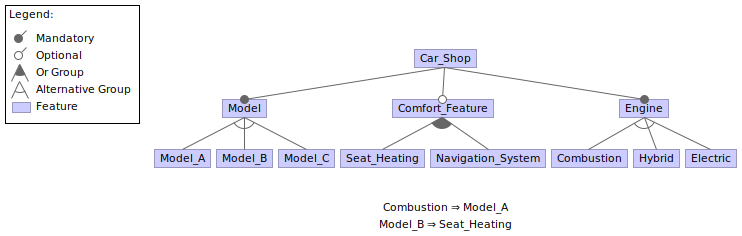
\includegraphics[scale=0.6]{gfx/Car_Shop.png}
    \caption{A feature model of a car shop}
    \label{fig:car}
\end{figure}

A configurable system often contains numerous features, all these features might interact with one another or have different dependencies.
To help us keep a overview of the system we introduce feature model \cite{Feature-Oriented-Software-Product-Lines-Feature-models}. A example
of a feature model for a car shop can be found in \ref{fig:car}

A feature model is essentialy a tree, that models a configurable system, each node in that tree represent a specific feature whereas the root
represent the system itself. If a feature is selected it implies that also the parent of that features needs to be selected as well, the further
we decend in the tree the more specific features get. In \ref{fig:car} we see Engine is a feature where as the children a concrete types
of engines, specificly Combustion, Hybrid and Electric.

Each feature may contain a grafical notation to indicate whether the feature is mandatory or optional, if the feature is mandatory, it is 
indicated with a black bubble and if its optional its optional its indicated with a empty bubble, in \ref{fig:car} we can see that Engine and
Model are mandatory features, which make sense since both are necessary for each car, but Comfort\_Feature a optional since they are not
necessary for a car to function.

Besides mandatory and optional feature we also have alternative and choice groups. A parent can have one of these groups, a alternative group
is denoted with a empty half circle and a optional group with a filled circle. If a choice group is used, one feature needs to be selected, but
others can be selected as well, a choice group corresponds to the logical or operator. In a alternative group, one and only one feature can be
selected, if more the one is selected the configuration is invalid. In \ref{fig:car} we see Engine has a alternative group, which makes sense
since each car can only contain one Engine, where it makes sense that Comfort\_Feature contains a choice group, you can have a navigation system
and seat heating in a car without any conflics.

In addition to that, a feature model can contain different constraints that need to be satisfied, these constraints are defined as boolean 
algebra. In \ref{fig:car} we can see that there are two constraints, $Combustion \implies Model\_A$ and 
$Model\_B \implies Seat\_Heating$, the reasons for such constraints could be that Model\_B is a luxurious model where it only gets shipped
with seat heating.

Every feature model can also be translated into compositional logic \cite*{Feature-Oriented-Software-Product-Lines-Feature-models}, therefore
configuration of features is only valid iff it satisfies the propositional logic. We can therefore use a feature model to check wheter a 
configuration is valid, which is especially useful if we want to sample or enumerate all valid configurations. 